%課題研究レジュメテンプレート ver. 1.2

\documentclass[uplatex]{jsarticle}
\usepackage[top=20mm,bottom=20mm,left=20mm,right=20mm]{geometry}
\usepackage[T1]{fontenc}
\usepackage{txfonts}
\usepackage{wrapfig}
\usepackage[expert,deluxe]{otf}
\usepackage[dvipdfmx,hiresbb]{graphicx}
\usepackage[dvipdfmx]{hyperref}
\usepackage{pxjahyper}
\usepackage{secdot}

\makeatletter
  \renewcommand{\section}{%
    \if@slide\clearpage\fi
    \@startsection{section}{1}{\z@}%
    {\Cvs \@plus.5\Cdp \@minus.2\Cdp}% 前アキ
    {.5\Cvs \@plus.3\Cdp}% 後アキ
    %{\normalfont\Large\headfont\raggedright}}
    {\normalfont\raggedright}}

  \renewcommand{\subsection}{\@startsection{subsection}{2}{\z@}%
    {\Cvs \@plus.5\Cdp \@minus.2\Cdp}% 前アキ
    {.5\Cvs \@plus.3\Cdp}% 後アキ
    %{\normalfont\large\headfont}}
    {\normalfont}}

  \renewcommand{\subsubsection}{\@startsection{subsubsection}{3}{\z@}%
    {\Cvs \@plus.5\Cdp \@minus.2\Cdp}%
    {\z@}%
    %{\normalfont\normalsize\headfont}}
    {\normalfont}}
\makeatother
%ここから上を編集する必要はない.





\title{\vspace{-14mm}ソーシャルゲームにおける登録数の増加と稼働日数の推移の関連性について}
\author{PMコース 矢吹研究室 1342029 遠藤一輝}
\date{}%日付を入れる必要はない.
\pagestyle{empty}%ページ番号は振らない.
\begin{document}
\maketitle





\section{研究の背景}% 629文字

技術が進歩していくにつれ,ゲームの種類も多様化してきている.その中の一形態として最近急激に数を増やした分野にソーシャルゲームがある.スマートフォンの性能の向上により本格的なゲームの動作にも耐え,携帯電話はゲーム機としての側面も持つようになった.
黎明期には複雑な操作を必要としない単純なゲームが多かったが,処理機能の向上によってゲーム内容もより複雑なものへとなっていった.
それはスマートフォンに搭載されたセンサーを有効に活用したものや,内容を深め戦略性やゲーム性を持たせたものであり,今や手軽に遊べるゲームから本格的なゲームまでその種類は多岐にわたる.\par
規模の拡大は凄まじい速度で進行しており,2007年にわずか4億円であった市場が2008年には48億円に,2009年には235億円となり,その後も2010年には1067億円,2011年には2000億円以上とその勢いはとどまることを知らない.\cite{shinbun}%引用1
だがその隆盛の裏には多くの失敗や挫折があり,様々な事情によりサービスを停止したゲームが多くあることも事実である.\par
ソーシャルゲームにとってヒットとなったかを測る指標として重要なのは登録人数である.
登録人数を増やすことは成功につながり,ソーシャルゲームを運営する上で意識しなければならない項目である.
ソーシャルゲームの数が増え,生存競争が激しくなった昨今では顧客を掴むためよりより魅力的なものにしていくことが重要である.
そのために傾向を掴み,それをもとに現状を改善しより多くの登録人数を得ることが必要となってくる.



\section{研究の目的}%83文字

ソーシャルゲームの登録人数および稼働日数の推移を調査し,パターンを分類する.
また,分析の結果を見ることによって今後のソーシャルゲームにおける登録人数の推移を予測するための指標とする.




\section{プロジェクトマネジメントとの関連}%94文字

稼働人数の推移を分析し今後の傾向を予測することで,改善案の早期立案がしやすくなる.また,増加の仕方から顧客の需要を予測することができる.以上の点からプロジェクトの成功率を高めることができる.



\section{研究の方法}%323文字

\subsection{可視化の方法}


ソーシャルゲームから公式によるアナウンスが行われた一定登録数突破の人数と突破日時を抜き出し,その推移を可視化する.稼働日数は稼働開始日から突破日までの日数とする.
可視化されたグラフから傾向をパターンごとに分類する.
その結果から進行中のソーシャルゲームについて今後の増加の傾向の予想を行う.


\subsection{条件}

抜き出すソーシャルゲームの条件として11月20日時点までに稼働開始しており,公式によるアナウンスがあるものに限る.


\subsection{サンプルの選出方法}

データのサンプルの選出についてはネットランキング\cite{octba}\cite{appget}の1位から10位までを抜き出し,それらゲームの中からソーシャルゲームのみを対象とする.サンプルの抽出を十数週にわたって行い,出てきたソーシャルゲームの中から無作為に選出する.


\begin{wrapfigure}[10]{r}{13cm}
\vspace*{-\intextsep}
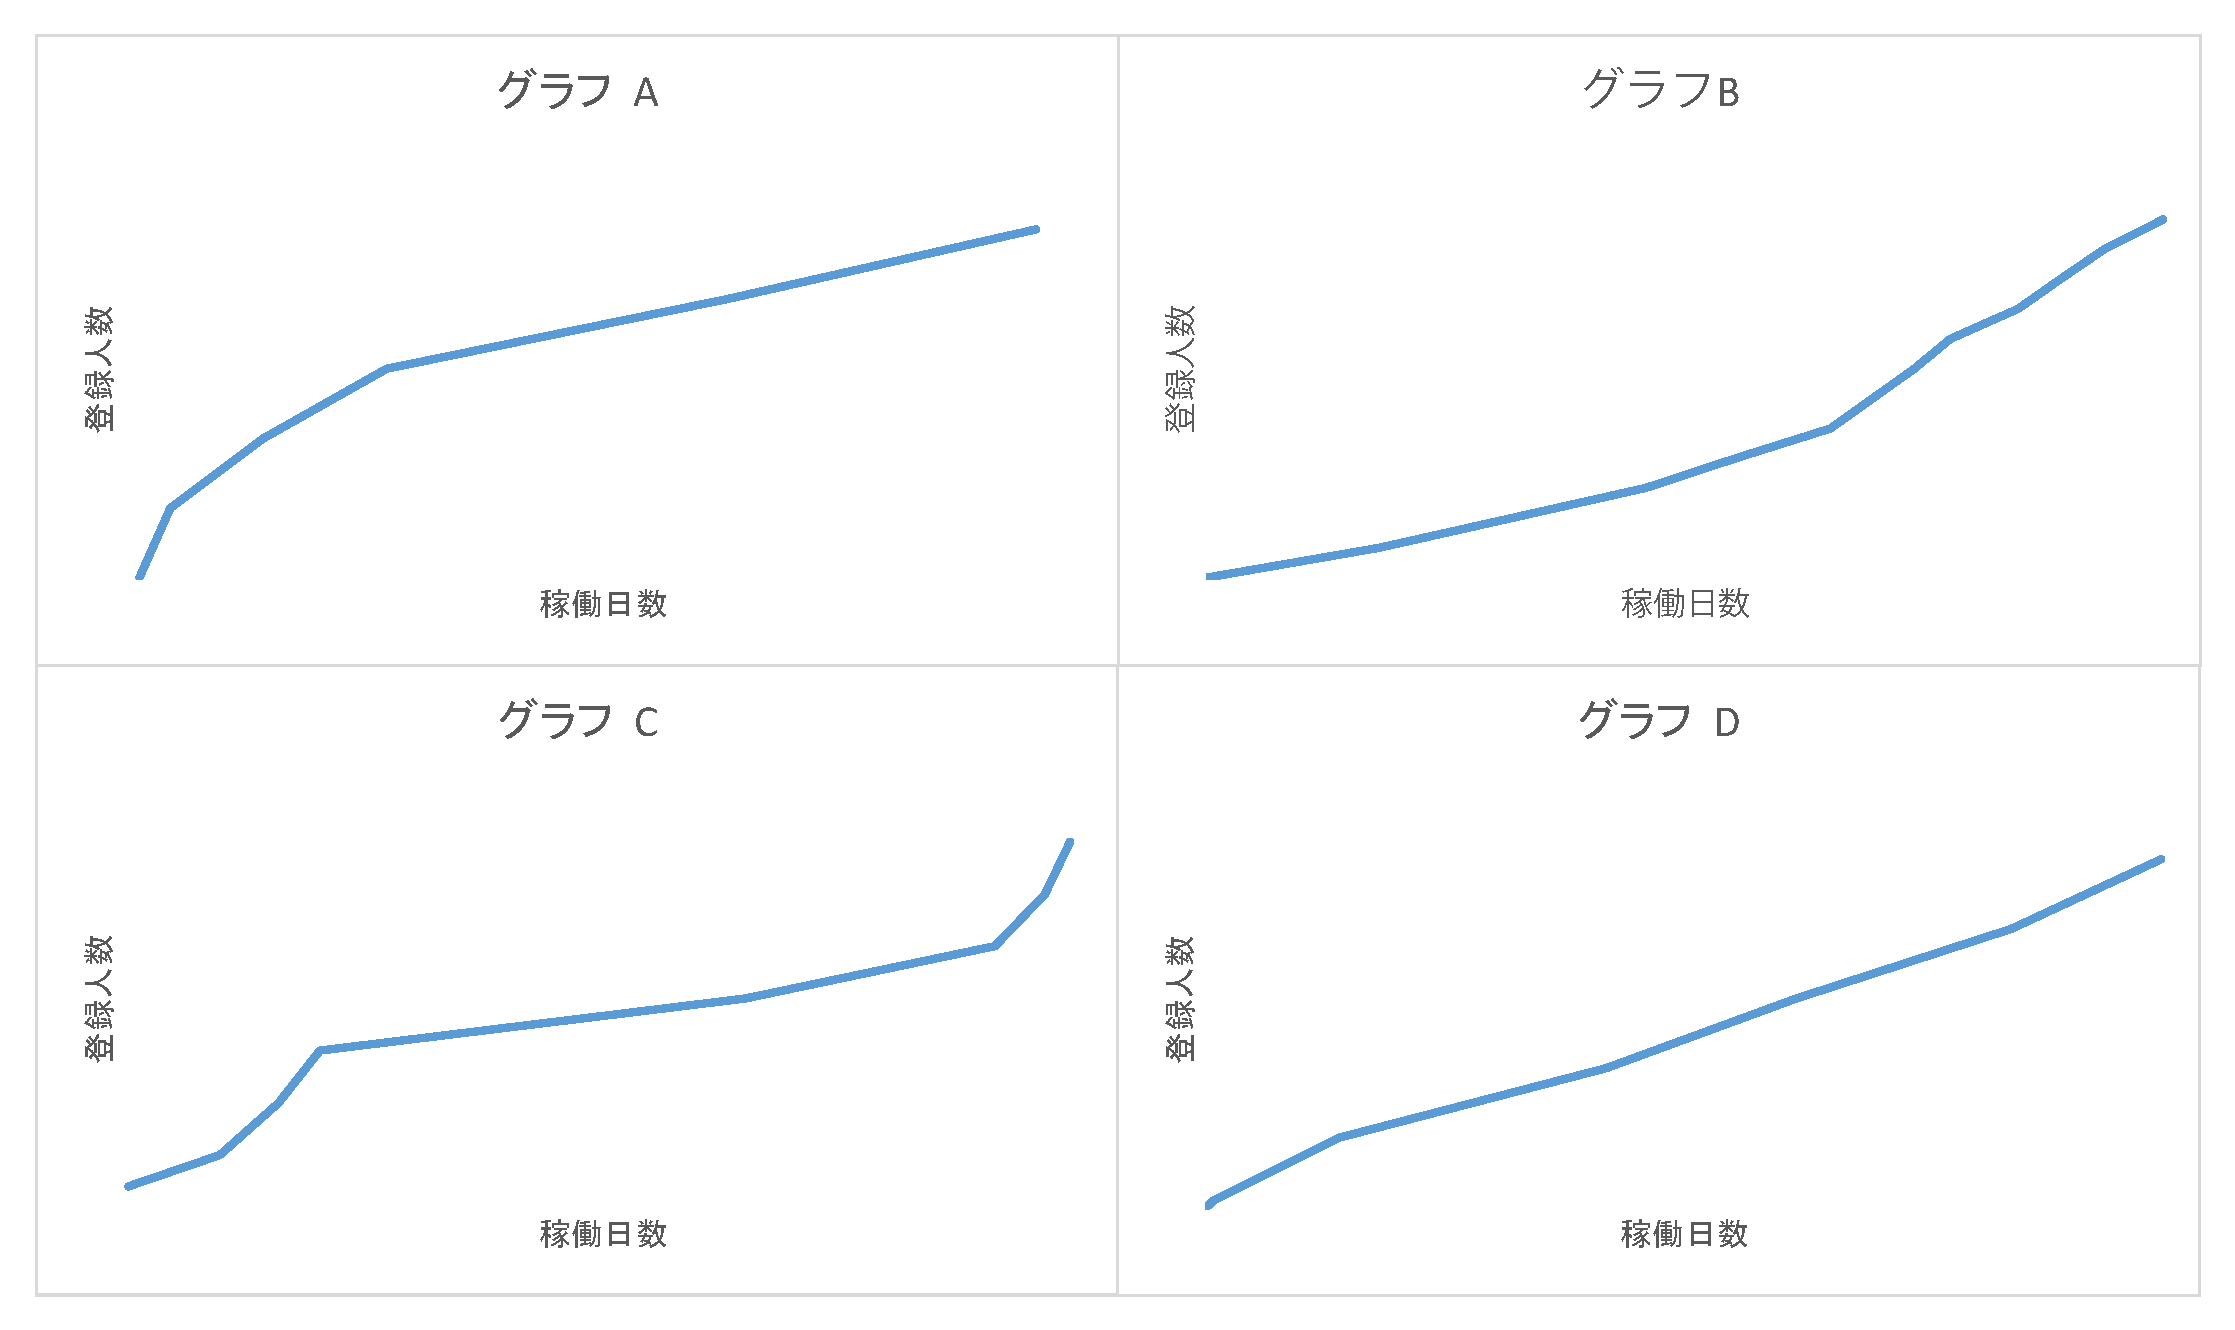
\includegraphics[width=11cm,clip]{g1.pdf}
\label{サンプル図}
\end{wrapfigure}


\section{現在の進捗状況}

分析のデータサンプルとして38件のソーシャルゲームを調査し,登録人数と稼働日数の推移について可視化を行った.可視化したグラフの傾向を元に,4つのパターンに分類した.


\begin{enumerate}
\item グラフA:
開始直後に急激に数値が伸び,以降緩やかになるパターンである.
ビッグタイトルや稼働前情報から期待の多く集まる作品に多かった伸び方である.
一方で稼働後のイメージとのギャップなどで失速するパターンも見られた.

\item グラフB:
序盤緩やかな傾斜を描くが,とある点を境に急激に上昇するパターンである.メディア進出やふとしたきっかけで人気が上昇し,その後も人気を保ち続ける後天的にビッグタイトルとなった作品の傾向である.開始直後は知名度が少ないがそれゆえにプレイヤーの作品に対するイメージが固まってないため,知名度が高くなって以降は安定して高い伸び方を続けることが多い.

\item グラフC:
不規則に急激な上昇と緩やかな上昇を繰り返すパターンである.
ある程度の知名度がある作品などがコラボレーションやメディア化によって急激に数を伸ばすが,その効果が薄れるにつれ上昇率も減衰し,緩やかな曲線を描くことになる.
その後別の案でそのサイクルを繰り返すため,不規則な推移になると考えられる.

\item グラフD:
平均的に伸び続けるパターンである.
口コミや宣伝で開始から安定して登録者数を伸ばし続ける.
今後の動向次第ではBのグラフのような曲線を描くこともある.

\end{enumerate}









\section{今後の計画}

以下のように研究を進める計画である.

\begin{enumerate}
\item データ件数を増やし,データの信頼性の向上を図る.
\item 4パターンについてより深い分析を行う.
\item 現行のゲームのグラフの推移から今後の推移を予測する.
\item 試行回数を増やし,制度の向上を図る.
\end{enumerate}


\bibliographystyle{junsrt}
\bibliography{biblio}%「biblio.bib」というファイルが必要.

\end{document}